\subsection{感度と相補感度}

閉ループ \weq{closed-loop} の開ループを $L(s)=C(s)G(s)$ とおく。単位負帰還の式
\begin{equation}
  u=C(r-y)
\end{equation}
と対象の式 $y=Gu$ を組み合わせると、
\begin{align}
  y&=GC(r-y),\\
  (1+GC)y&=GC\,r
\end{align}
である。したがって目標値から出力への伝達は
\begin{equation}
  T(s)=\frac{L(s)}{1+L(s)}
\end{equation}
である。この $T(s)$ を相補感度関数という。感度関数は
\begin{equation}
  S(s)=\frac{1}{1+L(s)}
\end{equation}
である。両者は
\begin{equation}
  S(s)+T(s)=1
\end{equation}
を満たす。

\subsubsection{目標値・外乱・測定ノイズの伝達経路}

感度関数と相補感度関数は、単なる記号ではなく、閉ループ内の信号経路を分けるための基本量である。入力側外乱 $d_u$、出力側外乱 $d_y$、測定ノイズ $n$ を
\begin{align}
  y&=G(u+d_u)+d_y,\\
  y_m&=y+n,\\
  u&=C(r-y_m)
\end{align}
で定義する。ここで $y_m$ は制御器に戻される測定値であり、$r$ は目標値である。上式を消去すると
\begin{align}
  y&=T r+G S d_u+S d_y-T n,\\
  e_y&=r-y=S r-G S d_u-S d_y+T n,\\
  u&=C S r-T d_u-C S d_y-C S n
\end{align}
を得る。符号は加え方の規約に依存するが、振幅の議論では $\abs{S}$、$\abs{T}$、$\abs{GS}$、$\abs{CS}$ が重要である。

低周波で $\abs{L(j\omega)}\gg1$ なら
\begin{equation}
  S(j\omega)\simeq \frac{1}{L(j\omega)},\qquad
  T(j\omega)\simeq 1
\end{equation}
である。したがって目標値は出力へよく伝わり、出力側外乱は $S$ により抑制される。一方、測定ノイズは出力へ $-T$ を通って現れるため、測定ノイズが大きい周波数帯で $T\simeq1$ にしておくと出力が測定ノイズを追いやすい。高周波で $\abs{L(j\omega)}\ll1$ なら
\begin{equation}
  S(j\omega)\simeq1,\qquad
  T(j\omega)\simeq L(j\omega)
\end{equation}
であり、測定ノイズから出力への伝達は小さくなるが、出力側外乱の抑制は弱くなる。ループ整形では、外乱や目標値の主成分がある低周波で $\abs{S}$ を下げ、測定ノイズや未モデル化共振がある高周波で $\abs{T}$ を下げるように $L$ の大きさと位相を選ぶ。

\subsubsection{モデル不確かさとロバスト安定性}

モデル $G(s)$ と実対象 $G_{\mathrm{p}}(s)$ が完全には一致しないとき、閉ループ安定性は名目モデルだけでは判断できない。乗法的不確かさは
\begin{equation}
  G_{\mathrm{p}}(s)=G(s)\{1+W_m(s)\Delta_m(s)\},
  \qquad
  \abs{\Delta_m(j\omega)}\le 1
\end{equation}
と表す。$W_m$ は周波数ごとの相対誤差の上限を表す重みであり、無次元である。このとき実対象を含む閉ループ特性方程式は
\begin{align}
  1+C(s)G_{\mathrm{p}}(s)
  &=1+L(s)+L(s)W_m(s)\Delta_m(s)\\
  &=(1+L(s))
    \{1+W_m(s)T(s)\Delta_m(s)\}
\end{align}
である。名目閉ループが安定であり、すべての周波数で
\begin{equation}
  \abs{W_m(j\omega)T(j\omega)}<1
\end{equation}
が成り立つなら、$\abs{\Delta_m}\le1$ の範囲で第 2 因子は 0 にならない。これは小ゲイン定理に基づく十分条件であり、入門的には「相対モデル誤差が大きい周波数では相補感度 $T$ を小さく保つ」という設計指針として読める。ナイキスト線図でいえば、モデル誤差によって開ループ点が動いても、点 $-1$ に届かないだけの距離を保つ条件である。

加法的不確かさは、絶対誤差を直接
\begin{equation}
  G_{\mathrm{p}}(s)=G(s)+W_a(s)\Delta_a(s),
  \qquad
  \abs{\Delta_a(j\omega)}\le1
\end{equation}
と書く。$W_a$ は対象の伝達関数と同じ単位を持つ。特性方程式は
\begin{align}
  1+C(s)G_{\mathrm{p}}(s)
  &=1+L(s)+C(s)W_a(s)\Delta_a(s)\\
  &=(1+L(s))
    \{1+C(s)S(s)W_a(s)\Delta_a(s)\}
\end{align}
であるから、対応する十分条件は
\begin{equation}
  \abs{C(j\omega)S(j\omega)W_a(j\omega)}<1
\end{equation}
である。乗法的不確かさは高周波の未モデル化極、柔軟モード、むだ時間のような相対誤差を扱いやすく、加法的不確かさは低周波のゲイン誤差や未測定の並列経路を絶対誤差として扱いやすい。

\subsubsection{Bode の感度積分とウォーターベッド効果}

$S+T=1$ であるため、同じ周波数で $S$ と $T$ を同時に任意に小さくすることはできない。さらに安定なフィードバックには、周波数全体にわたる制約がある。たとえば、閉ループが安定で、開ループが有理関数で、感度積分の標準的な仮定を満たすとき、Bode の感度積分は概略
\begin{equation}
  \int_0^\infty \log\abs{S(j\omega)}\,\dd\omega
  =\pi\sum_{p_i\in\mathbb{C}_+}\operatorname{Re}p_i
\end{equation}
と書ける。和は開ループの右半平面極 $p_i$ について取る。開ループが安定で右半平面極を持たない場合、右辺は 0 になる。したがって、ある周波数帯で $\abs{S}<1$ として外乱を抑えると、別の周波数帯では $\abs{S}>1$ となる領域が生じる。この性質をウォーターベッド効果という。不安定極がある場合には右辺が正になり、感度の盛り上がりをより強く要求する。

この積分式は、入門段階では厳密な設計公式というより、ループ整形の限界を示す原理として使う。低周波で外乱抑制を強めるほど、交差周波数付近の感度ピーク
\begin{equation}
  M_s=\max_{\omega\ge0}\abs{S(j\omega)}
\end{equation}
が大きくなりやすい。$M_s$ が大きいことは、ナイキスト線図が点 $-1$ に近づくことと同じ意味を持ち、モデル誤差、外乱、パラメータ変動に対する余裕が小さいことを表す。

\wfig{frequency-design-examples} 下段は、開ループ
\begin{equation}
  L_K(s)=\frac{K}{s(s+1)}
\end{equation}
で $K=0.3,1,3$ を比較したものである。$K$ を大きくすると低周波の $\abs{S}$ は下がり、出力側外乱や低周波の追従誤差は抑えやすくなる。一方で、交差周波数付近の $M_s$ は大きくなり、$\abs{T}$ が $0\,\mathrm{dB}$ 近くに残る帯域も高周波側へ広がる。測定ノイズや未モデル化の高周波モードがその帯域にある場合、低周波の性能改善がロバスト性やノイズ感度の悪化として戻ってくる。

\begin{figure}[tbp]
\centering
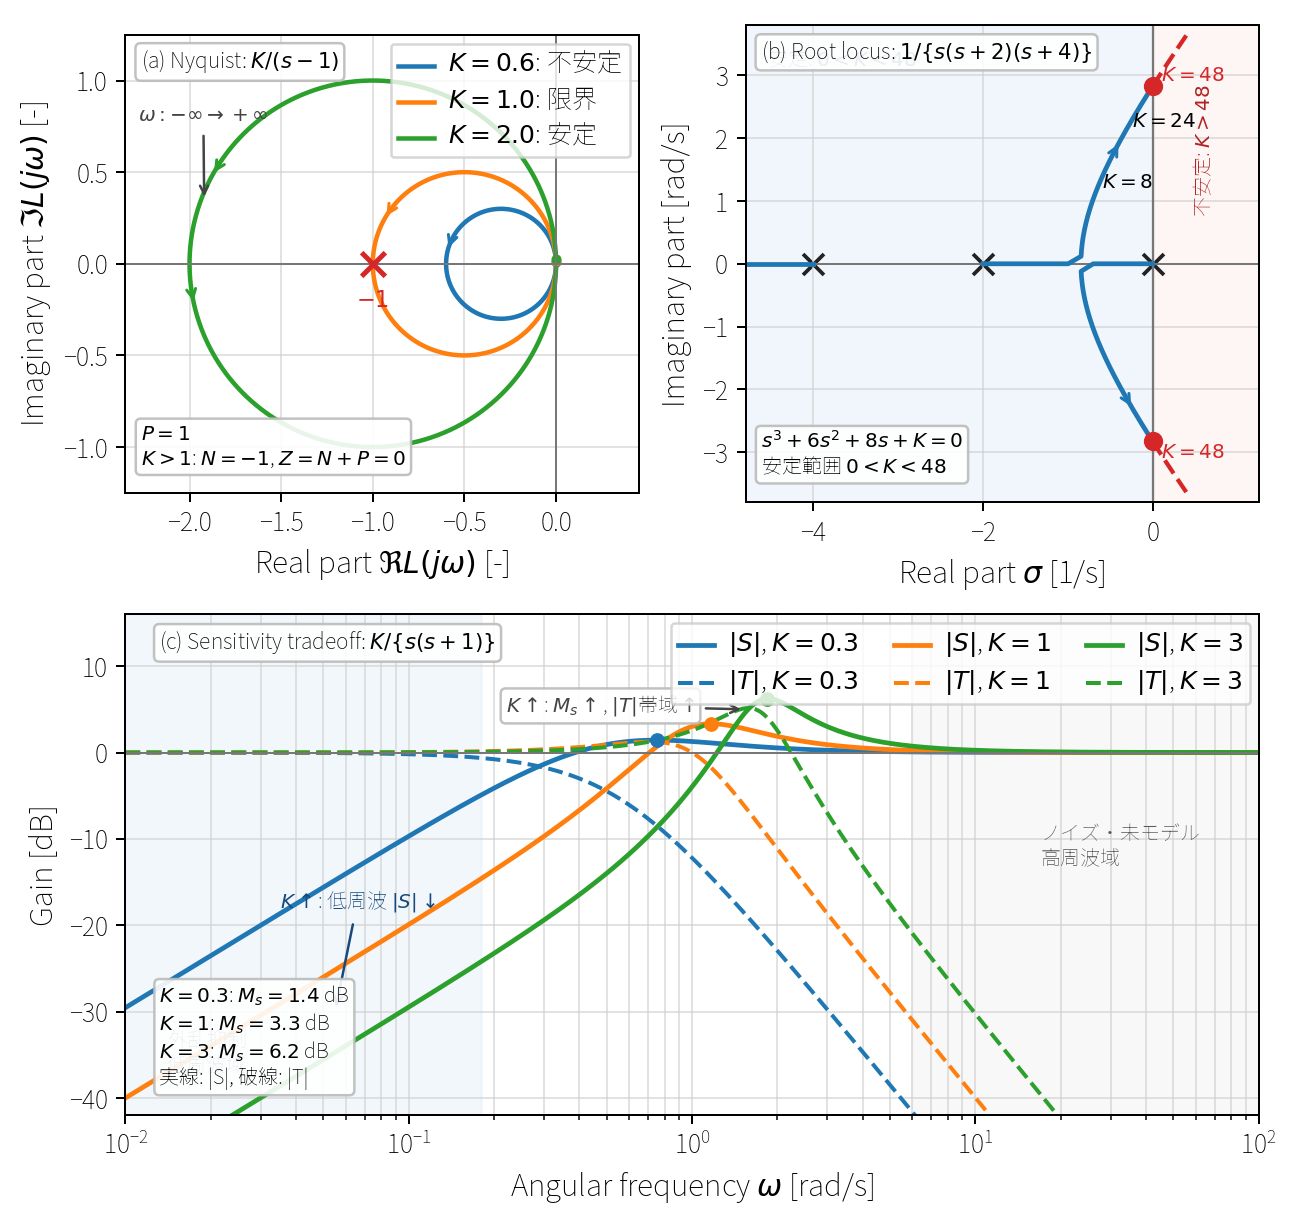
\includegraphics[width=0.96\linewidth,bb=0 0 1296 1224]{figures/frequency_design_examples.png}
\caption{ナイキスト線図、根軌跡、感度関数を同じ周波数設計の確認図として並べた例。上左は不安定開ループ極 $P=1$ を持つ $L_K(s)=K/(s-1)$ のゲイン変化で、$K>1$ だけが点 $-1$ を反時計回りに 1 回囲み閉ループが安定になる。上右は三次開ループ $G(s)=1/\{s(s+2)(s+4)\}$ の根軌跡で、$0<K<48$ が安定範囲、$K=48$ で虚軸を横切る。下は $L_K(s)=K/\{s(s+1)\}$ の $S$ と $T$ で、ゲインを上げるほど低周波の外乱抑制は強くなるが、感度ピークと相補感度の通過帯域が増える。}
\label{fig:frequency-design-examples}
\end{figure}

\begin{practice}[周波数設計図による安定性と感度の確認]
\wfig{frequency-design-examples} を用いる。上左で $K=0.6,1,2$ の各曲線について $N$、$P$、$Z$ を対応させ、上右で $K=48$ が安定限界になることを Routh 表の第一列と結びつけよ。最後に、下段の $K=0.3,1,3$ を比べ、低周波の $\abs{S}$、感度ピーク $M_s$、高周波側の $\abs{T}$ のどれが改善し、どれが悪化するかを一文ずつ述べよ。
\end{practice}

\subsubsection{むだ時間による位相損失}

むだ時間 $\tau_d$ を含む対象は、名目対象に $e^{-s\tau_d}$ が掛かった形で表される。周波数応答では
\begin{equation}
  \abs{e^{-j\omega\tau_d}}=1,\qquad
  \angle e^{-j\omega\tau_d}=-\omega\tau_d
\end{equation}
であり、ゲインを変えずに位相だけを遅らせる。ゲイン交差周波数 $\omega_{gc}$ の近くで安定余裕が決まる場合、位相余裕 $\phi_m$ をラジアンで表せば、むだ時間余裕の近似は
\begin{equation}
  \tau_{d,\max}\simeq\frac{\phi_m}{\omega_{gc}}
\end{equation}
である。交差周波数を高くして速い応答を得るほど、同じ位相余裕から得られるむだ時間余裕は短くなる。

むだ時間は乗法的不確かさとしても読める。むだ時間を無視した名目モデル $G(s)$ に対し、実対象が $G(s)e^{-s\tau_d}$ であるなら
\begin{equation}
  G(s)e^{-s\tau_d}
  =G(s)\{1+(e^{-s\tau_d}-1)\}
\end{equation}
である。したがって乗法誤差の大きさは
\begin{equation}
  \abs{e^{-j\omega\tau_d}-1}
  =2\abs{\sin\frac{\omega\tau_d}{2}}
  \simeq \omega\tau_d
  \qquad (\omega\tau_d\ll1)
\end{equation}
となる。高周波ほどむだ時間の相対誤差は大きくなるため、ロバスト安定条件 $\abs{W_mT}<1$ は高周波で $T$ を小さくする必要を与える。複数のゲイン交差や大きな共振ピークがある場合には、上の近似式だけでなくナイキスト線図または閉ループ極で確認する。

\begin{example}[一次対象の感度とむだ時間余裕]
一次対象
\begin{equation}
  G(s)=\frac{1}{s+1}
\end{equation}
を積分器 $C(s)=1/s$ で単位負帰還制御する。開ループは
\begin{equation}
  L(s)=\frac{1}{s(s+1)}
\end{equation}
であり、
\begin{equation}
  S(s)=\frac{s(s+1)}{s(s+1)+1},
  \qquad
  T(s)=\frac{1}{s(s+1)+1}
\end{equation}
である。低周波 $\omega=0.1\,\mathrm{rad/s}$ では $\abs{L(j\omega)}\simeq9.95$ なので、$\abs{S(j\omega)}$ はおよそ $0.1$、$\abs{T(j\omega)}$ はおよそ 1 である。目標値追従と低周波外乱抑制はよいが、同じ低周波に含まれる測定ノイズは出力へ通りやすい。

交差周波数は
\begin{equation}
  \frac{1}{\omega\sqrt{1+\omega^2}}=1
\end{equation}
から
\begin{equation}
  \omega_{gc}
  =\sqrt{\frac{\sqrt{5}-1}{2}}
  \simeq0.786\,\mathrm{rad/s}
\end{equation}
である。このとき開ループ位相は
\begin{equation}
  \angle L(j\omega_{gc})
  =-90^\circ-\tan^{-1}(0.786)
  \simeq-128.2^\circ
\end{equation}
なので、位相余裕は
\begin{equation}
  \phi_m\simeq51.8^\circ
  =0.904\,\mathrm{rad}
\end{equation}
である。むだ時間余裕の近似は
\begin{equation}
  \tau_{d,\max}\simeq\frac{0.904}{0.786}
  \simeq1.15\,\mathrm{s}
\end{equation}
となる。

交差周波数付近では感度が盛り上がる。たとえば $\omega=1\,\mathrm{rad/s}$ では
\begin{equation}
  L(j)=\frac{1}{j(1+j)}=-\frac{1}{2}-\frac{1}{2}j
\end{equation}
であるから
\begin{equation}
  \abs{S(j)}
  =\frac{1}{\abs{1+L(j)}}
  =\sqrt{2},\qquad
  \abs{T(j)}=1
\end{equation}
となる。低周波で $\abs{S}$ を下げた代償として、交差周波数付近に $\abs{S}>1$ の帯域が現れている。乗法誤差の上限がこの周波数帯で $\abs{W_m}\le0.3$ なら、少なくともこの点では $\abs{W_mT}\le0.3<1$ であり、乗法誤差だけから見ると余裕がある。一方、むだ時間が $1\,\mathrm{s}$ に近づくと交差周波数で約 $45^\circ$ の位相を失い、残りの位相余裕は小さい。応答を速くするためにゲインを上げれば $\omega_{gc}$ が上がり、同じむだ時間に対する位相損失はさらに大きくなる。
\end{example}
